\section{Results}\label{sec:results}

\subsection{Spread under residual aberrations}

Table~\ref{tab:main} gives, for each of the \nSeedsAll{} seeds of the holograms, the 95th percentile of the relative standard deviation over the ensemble of \parNens{} aberration draws for phase-fixed WGS and for the robust hologram, their ratio $\rho$ with the paired bootstrap interval over the draws, the efficiency ratio $\eta$, and the number of draws on which the robust hologram has the lower spread. On the three seeds of the acceptance test the median ratio is
\ratioMed{} (range \ratioMin{} to \ratioMax) at a median efficiency ratio of \effRatioMed{} (\effRatioMin{} to \effRatioMax); over all \nSeedsAll{} seeds the median is \ratioAllMed{} with a bootstrap interval of the median from \ratioAllCiLo{} to \ratioAllCiHi, and the efficiency ratio stays between \effAllMin{} and \effAllMax. Hypothesis H1 holds on \seedsPassing{} of \nSeedsAll{} seeds and H2 on \seedsEffPassing{} of \nSeedsAll.
The bootstrap intervals of single seeds are wide, from about \ratioOneLo{} to \ratioOneHi{} for seed 1, and \ciBelowN{} of the \nSeedsAll{} intervals have a lower end under $1.25$: the criterion is met by every seed's point estimate and by the median over seeds, not by every interval of a single $200$-draw ensemble.

\begin{table}[t]
\centering\small
\caption{Spread under residual aberrations on the $10\times10$ task: 95th percentile of the relative standard deviation (percent) over 200 draws for phase-fixed WGS and for the robust hologram, their ratio with the 95 percent paired bootstrap interval over the draws, the efficiency ratio, and the draws on which the robust hologram has the lower spread, for each seed of the holograms.}
\label{tab:main}
\begin{tabular}{@{}r r r l r r@{}}
\toprule
Seed & $Q_{95}$ WGS & $Q_{95}$ robust & $\rho$ [interval] & $\eta$ & draws won\\
\midrule
1 & 6.192 & 3.947 & 1.57 [1.34, 1.73] & 0.981 & 200/200 \\
2 & 5.983 & 4.220 & 1.42 [1.29, 1.70] & 0.983 & 200/200 \\
3 & 6.068 & 4.230 & 1.43 [1.27, 1.61] & 0.982 & 200/200 \\
4 & 5.925 & 4.050 & 1.46 [1.28, 1.65] & 0.983 & 200/200 \\
5 & 5.923 & 4.376 & 1.35 [1.27, 1.66] & 0.982 & 200/200 \\
6 & 5.955 & 3.906 & 1.52 [1.21, 1.62] & 0.982 & 200/200 \\
7 & 6.080 & 4.151 & 1.46 [1.26, 1.64] & 0.982 & 200/200 \\
8 & 5.965 & 4.362 & 1.37 [1.31, 1.64] & 0.982 & 200/200 \\
9 & 5.948 & 4.312 & 1.38 [1.29, 1.64] & 0.982 & 200/200 \\
10 & 5.856 & 4.056 & 1.44 [1.23, 1.61] & 0.982 & 200/200
\\
\midrule
Median, seeds 1 to 3 & & & \ratioMed{} (\ratioMin{} to \ratioMax) & \effRatioMed & \\
Median, \nSeedsAll{} seeds & & & \ratioAllMed{} [\ratioAllCiLo, \ratioAllCiHi] & \effAllMed & \\
\bottomrule
\end{tabular}
\end{table}

Figure~\ref{fig:ecdf} shows the whole distribution for seed 1. The robust hologram has the lower spread on \winsOne{} of the \parNens{} draws (exact sign test, $p=\signPOne$), its median spread is \evalMedBfour{} percent against \evalMedNom{}, its mean \evalMeanBfour{} against \evalMeanNom, and its largest spread \evalMaxBfour{} against \evalMaxNom{} percent. The whole distribution moves left, so the gain is not confined to the tail that the 95th percentile selects; the ratio of the means is \meanRatioOne{} on this seed, a little larger than the ratio of the 95th percentiles of \ratioOne.
Figure~\ref{fig:seeds} shows the ratio and the efficiency ratio for every seed: the ratios range from \ratioAllMin{} to \ratioAllMax{} and the efficiency ratio is within \effAllMin{} to \effAllMax, a seed-to-seed variation of the design that is small against the gain.

\begin{figure}[t]
\centering
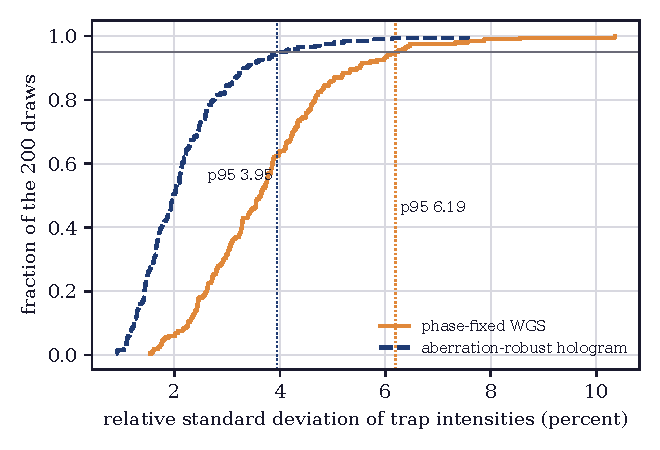
\includegraphics[width=0.62\textwidth]{fig-ecdf.pdf}
\caption{Empirical distribution function over the 200 aberration draws of the relative standard deviation of the 100 trap intensities (percent), for phase-fixed WGS (solid) and the robust hologram (dashed), seed 1. The dotted verticals mark the 95th percentiles, the horizontal line the 95 percent level.}
\label{fig:ecdf}
\end{figure}

\begin{figure}[t]
\centering
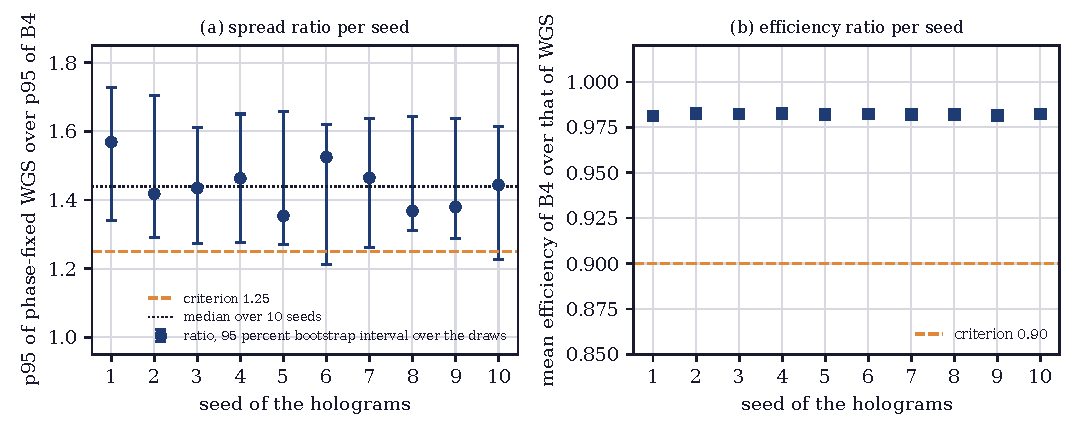
\includegraphics[width=\textwidth]{fig-seeds.pdf}
\caption{(a) Ratio of the 95th percentiles of phase-fixed WGS and of the robust hologram for each of ten seeds of the holograms, with the paired bootstrap interval over the 200 draws, the criterion of 1.25 and the median over seeds. (b) Ratio of the mean efficiencies over the ensemble with the criterion of 0.90.}
\label{fig:seeds}
\end{figure}

\subsection{Published methods on the same ensemble}

Table~\ref{tab:pub} scores the published methods that the product runs on the same task, the same seeds and the same ensemble; the entries are medians over the first three seeds. Weighted GS and phase-fixed WGS have the same 95th percentile at this iteration count (the ratio of the two is \pubGSWRatio), the Wirtinger gradient method with Adam reaches \pubWirtRatio{} of it, and these three are the only ones whose nominal spread is below one percent in the last column or close to it. Plain Gerchberg--Saxton,
the generalized adaptive additive variant and conjugate gradient started from the random superposition have nominal spreads of 18, 13 and 34 percent in the last column of the table at the budgets of the comparison (30, 30 and 40 iterations; the conjugate-gradient run has not converged and its efficiency is \pubCGEff{} of that of phase-fixed WGS), and so their spread under aberration is dominated by their nominal spread and a ratio against them is not informative about aberration. The robust hologram, which starts
from the phase-fixed WGS hologram and adds $\parIters$ conjugate-gradient iterations, is the only method of the table whose spread under aberration is below the baseline's by more than the criterion. H3 is also tested by the control of the ablation (Table~\ref{tab:abl}): the same conjugate gradient with the nominal cost, started from the same hologram, gives a ratio of \ablNominalMed{} (\ablNominalMin{} to \ablNominalMax), that is a larger spread than the baseline, at an efficiency ratio of \ablNominalEff. The expected cost, and not the iterations, produces the gain.

\begin{table}[t]
\centering\small
\caption{Published methods and the robust hologram on the same task and ensemble: median over seeds 1 to 3 of the 95th percentile and the mean of the relative standard deviation over the 200 aberration draws (percent), the mean efficiency over the ensemble, and the spread at the nominal system (percent).}
\label{tab:pub}
\begin{tabular}{@{}l r r r r@{}}
\toprule
Method & $Q_{95}$ & mean $\sigma$ & efficiency & nominal $\sigma$\\
\midrule
Gerchberg--Saxton & 19.25 & 18.41 & 0.739 & 18 \\
generalized adaptive additive & 14.55 & 13.52 & 0.736 & 13 \\
weighted GS & 6.06 & 3.70 & 0.732 & 0.74 \\
phase-fixed WGS & 6.07 & 3.63 & 0.721 & 0.015 \\
conjugate gradient, nominal cost & 35.16 & 34.40 & 0.266 & 34 \\
Wirtinger gradient with Adam & 6.34 & 4.18 & 0.714 & 2 \\
aberration-robust hologram & 4.22 & 2.16 & 0.709 & 1
\\
\bottomrule
\end{tabular}
\end{table}

\subsection{New draws of the prior and the cases of the committed bake}

The holograms of seeds 1 to 3 were scored on five ensembles of other seeds (1001 to 1005), each of 200 new draws of the same prior. The $\heldN$ ratios have a median of \heldMed{} and range from \heldMin{} to \heldMax, at a median efficiency ratio of \heldEffMed. The acceptance ensemble is therefore not the one that favours the method: the ratios on new ensembles are higher than on the acceptance ensemble, and the lowest of them is above the criterion.

The committed bake of the product runs the same methods on its cases, each with its own optics, and holds the relative standard deviation of one realization per seed. Table~\ref{tab:bake} and Fig.~\ref{fig:bake} show the five cases for which the robust hologram is baked. In the aberrated case, whose optics carry a stated aberration, the mean spread is \bakeNineB{} percent for the robust hologram against \bakeNineM{} for phase-fixed WGS, a ratio of \bakeNineRatio{} at \bakeNineEff{} of its efficiency; this is the ratio of means of one realization per seed and not the ratio of 95th percentiles over an ensemble, which is why it is smaller than the main result. On the cases without aberration the picture reverses: the robust hologram has a spread of 0.4 to 1.0 percent where phase-fixed WGS is below 0.01 percent in \bakeIdealBelow{} of \bakeIdealN{} case and seed pairs, and on the case limited by the device model both are near 13 percent. The nominal price of robustness is a small residual spread, visible in the first rows of the table.

\begin{table}[t]
\centering\small
\caption{Committed bake of the studio: mean over three seeds of the relative standard deviation of the trap intensities (percent) for phase-fixed WGS and for the robust hologram, the range of the latter over the seeds, and the mean efficiencies, for the five cases on which the robust hologram is baked. Each case has its own optics.}
\label{tab:bake}
\begin{tabular}{@{}l r r l r r@{}}
\toprule
Case & $\sigma$ WGS & $\sigma$ robust & range robust & $e$ WGS & $e$ robust\\
\midrule
C01 square grid & 0.004 & 0.586 & 0.42 to 0.77 & 0.788 & 0.777 \\
C02 grid feedback & 0.377 & 0.852 & 0.83 to 0.87 & 0.792 & 0.778 \\
C07 high na & 0.004 & 0.983 & 0.94 to 1.02 & 0.785 & 0.766 \\
C08 device limited & 13.215 & 12.948 & 12.53 to 13.56 & 0.678 & 0.670 \\
C09 aberrated & 6.164 & 5.309 & 4.59 to 5.83 & 0.447 & 0.443
\\
\bottomrule
\end{tabular}
\end{table}

\begin{figure}[t]
\centering
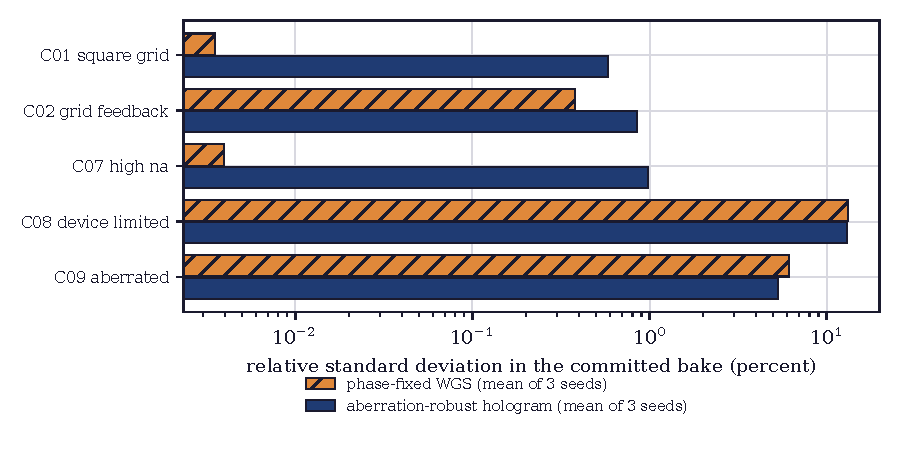
\includegraphics[width=0.78\textwidth]{fig-bake.pdf}
\caption{Relative standard deviation of the trap intensities (percent, logarithmic axis) of phase-fixed WGS and of the robust hologram on the five cases of the committed bake that include the robust hologram; mean of three seeds per case, each case with its own optics.}
\label{fig:bake}
\end{figure}

\subsection{Ensembles that differ from the design prior}

Table~\ref{tab:mismatch} and Fig.~\ref{fig:mismatch} score the same holograms, designed for eight modes at \parAb{} waves, on ensembles that differ from the prior: the same standard-normal draws scaled to other amplitudes, and ensembles with additional modes (Noll 12 to 15, and Noll 12 to 21) that the design did not include. For amplitudes below the design the ratio is \misBMed{} at 0.01 waves per mode, above the criterion, and \misAMed{} at 0.005, just below it; the ratio is limited at the lowest amplitude by the nominal spread of the robust hologram, about \thSigmaZeroBfour{} percent against \thSigmaZeroNom{} percent for the baseline. Above the design amplitude the gain falls to
\misDMed{} at 0.03 and \misEMed{} at 0.04 waves per mode. With modes outside the design the ratio is \misFMed{} when four more modes are added and \misGMed{} when the whole set up to Noll 21 is present: the design does nothing for modes it did not see. H7 therefore holds for smaller amplitudes and fails for larger ones and for other modes. The robust hologram is robust to the distribution it was designed for, and a measured residual that differs needs its own prior.

\begin{table}[t]
\centering\small
\caption{Holograms of seeds 1 to 3 on ensembles that differ from the design prior of 0.02 waves per mode over Noll 4 to 11: the 95th percentile of the spread (percent) of phase-fixed WGS and of the robust hologram (medians), the ratio with the range over the seeds, and the efficiency ratio.}
\label{tab:mismatch}
\begin{tabular}{@{}l r r l r@{}}
\toprule
Evaluation ensemble & $Q_{95}$ WGS & $Q_{95}$ robust & $\rho$ (range) & $\eta$\\
\midrule
0.005 waves per mode, Noll 4 to 11 & 1.42 & 1.13 & 1.24 (1.22 to 1.34) & 0.981 \\
0.01 waves per mode, Noll 4 to 11 & 2.85 & 1.65 & 1.75 (1.72 to 1.77) & 0.981 \\
0.02 waves per mode, Noll 4 to 11 & 6.07 & 4.22 & 1.43 (1.42 to 1.57) & 0.982 \\
0.03 waves per mode, Noll 4 to 11 & 10.01 & 8.60 & 1.16 (1.06 to 1.20) & 0.983 \\
0.04 waves per mode, Noll 4 to 11 & 15.17 & 14.82 & 1.02 (0.99 to 1.03) & 0.985 \\
design modes plus 12 to 15 added & 6.64 & 5.40 & 1.22 (1.19 to 1.24) & 0.983 \\
design modes plus Noll 12 to 21 & 10.66 & 10.63 & 0.99 (0.97 to 1.02) & 0.984
\\
\bottomrule
\end{tabular}
\end{table}

\begin{figure}[t]
\centering
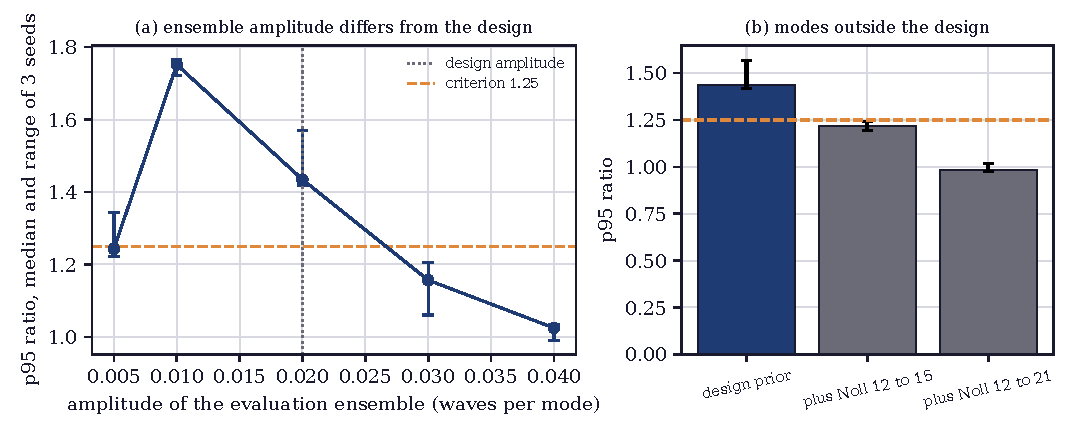
\includegraphics[width=\textwidth]{fig-mismatch.pdf}
\caption{(a) Ratio of the 95th percentiles against the amplitude of the evaluation ensemble, for holograms designed at 0.02 waves per mode; median and range of three seeds. (b) The same ratio on the design prior and on ensembles that add Noll modes 12 to 15 and 12 to 21 at 0.02 waves per mode.}
\label{fig:mismatch}
\end{figure}

\subsection{Check of the first-order theory}

Table~\ref{tab:theory} and Fig.~\ref{fig:theory} test Proposition 3 on the three seeds. The first-order response matrix $G$ was computed by central differences of $\pm10^{-3}$ waves in each of the eight modes at the nominal system, and the spread of each of the 200 draws was predicted from it. For phase-fixed WGS the prediction follows the draws closely: the Pearson correlation between the predicted and the measured spread is \thPearsonNom, the predicted mean squared spread is \thPredSqNom{} against \thMeasSqNom{} measured, and the 95th percentile is \thQLinNom{} against \thQMeasNom{} percent. For the robust hologram the correlation is
\thPearsonBfour, the predicted mean squared spread is \thPredSqBfour{} against \thMeasSqBfour{} measured, and the predicted 95th percentile is \thQLinBfour{} against \thQMeasBfour{}. H5 is met for the baseline and not for the robust hologram, by either of its two parts: the correlation is below $0.9$ and the measured mean squared spread exceeds the first-order value on both holograms (the first-order value is an approximation and not a strict bound, since it neglects the second-order terms of the response).
The first-order intensity variance $s^2\sum G^2$ falls by a factor of \thPRatio{} from the baseline to the robust hologram, so the first-order model predicts a ratio of 95th percentiles of about \thQLinRatio{} where the measurement gives \ratioMed. The optimizer removes most of the first-order response, and the spread that remains in the ensemble is mostly second order in the aberration, which the sigma points reach only through the second derivatives (Proposition 1).

\begin{table}[t]
\centering\small
\caption{Check of the first-order model of the spread (Proposition 3) for each seed and hologram: nominal spread $\sigma_0$ (percent), measured mean squared spread over the 200 draws, the value $\sigma_0^2+s^2\operatorname{tr}\Gamma$, the uncentred bound of Eq.~\eqref{eq:spreadbound}, the Pearson correlation between predicted and measured spread per draw, and the measured and predicted 95th percentiles (percent).}
\label{tab:theory}
\small
\begin{tabular}{@{}r l r r r r r r r@{}}
\toprule
Seed & Hologram & $\sigma_0$ & measured $\overline{\sigma^2}$ & first order & bound & Pearson & $Q_{95}$ & $Q_{95}$ first order\\
\midrule
1 & phase-fixed WGS & 0.0093 & 15.88 & 14.78 & 14.78 & 0.983 & 6.19 & 5.82 \\
1 & B4 & 0.88 & 5.78 & 4.11 & 4.11 & 0.897 & 3.95 & 2.89 \\
2 & phase-fixed WGS & 0.37 & 14.87 & 13.59 & 13.59 & 0.978 & 5.98 & 5.68 \\
2 & B4 & 1 & 5.39 & 3.73 & 3.74 & 0.877 & 4.22 & 2.68 \\
3 & phase-fixed WGS & 0.015 & 14.86 & 13.40 & 13.40 & 0.974 & 6.07 & 5.70 \\
3 & B4 & 1 & 5.66 & 3.81 & 3.82 & 0.867 & 4.23 & 2.79
\\
\bottomrule
\end{tabular}
\end{table}

Table~\ref{tab:cost} decomposes the robust cost of Proposition 2 at the level $\ell=\parLevel$. The nominal cost $L_0$ of the baseline is \thLzeroNom, the sigma-point average $J_{\mathcal S}$ is \thJsigNom, and the difference $J_{\mathcal S}-L_0$ is \thDeltaJNom, negative; the Gauss--Newton term is \thGNNom, positive and small, so the residual term of Eq.~\eqref{eq:curvature} is the large one, of size \thResidNom. The reason is that the level is a fraction of the start efficiency: aberrations lower the mean intensity of the traps toward the target (the start efficiency is
\startEffOne{} and the mean efficiency over the ensemble is \effDropOne{} of it, close to the exponential approximation of the Strehl ratio, \strehlExp), so the expected cost of the baseline is lower than its nominal cost. The level of $\ell=\parLevel$ thus encodes the expected loss of mean intensity, which is why the ablation of the level in Section~\ref{sec:ablation} has its maximum there, and the robust cost lowers $J_{\mathcal S}$ further, to \thJsigBfour{} for the robust hologram.

\begin{figure}[t]
\centering
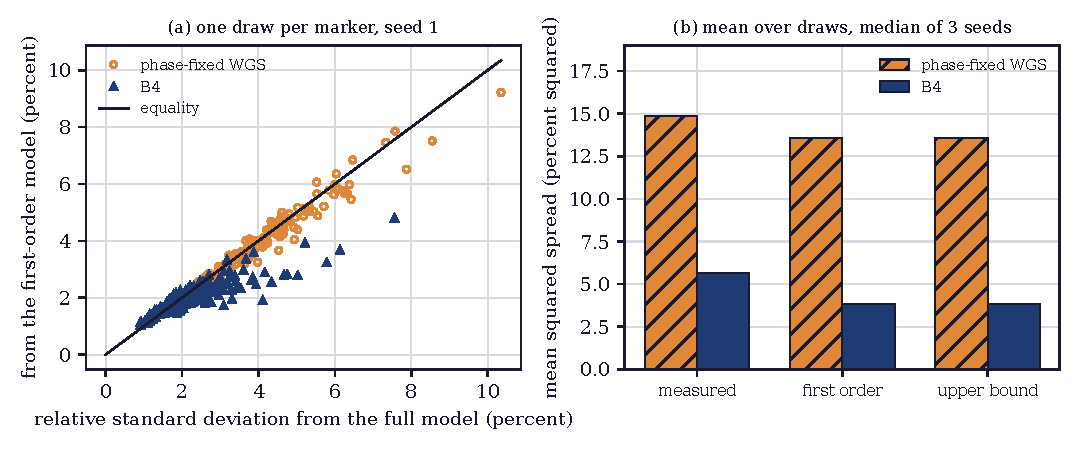
\includegraphics[width=\textwidth]{fig-theory.pdf}
\caption{(a) Relative standard deviation of each of the 200 draws predicted by the first-order model of the response against the value computed with the full model, for phase-fixed WGS and the robust hologram (seed 1). (b) Mean squared relative standard deviation over the draws: measured, first-order value and uncentred bound, median of three seeds.}
\label{fig:theory}
\end{figure}

\begin{table}[t]
\centering\small
\caption{Decomposition of the expected cost for each seed and hologram at the level used by the robust hologram: nominal cost $L_0$, sigma-point average $J_{\mathcal S}$, their difference, and the Gauss--Newton term $s^2\sum G^2/T_\Sigma$ of Eq.~\eqref{eq:curvature}.}
\label{tab:cost}
\begin{tabular}{@{}r l r r r r@{}}
\toprule
Seed & Hologram & $L_0$ & $J_{\mathcal S}$ & $J_{\mathcal S}-L_0$ & Gauss--Newton\\
\midrule
1 & phase-fixed WGS & 0.0123 & 0.00194 & $-$0.0104 & 0.00183 \\
1 & robust hologram & 0.00799 & 0.000743 & $-$0.00724 & 0.000395 \\
2 & phase-fixed WGS & 0.0124 & 0.00185 & $-$0.0105 & 0.00166 \\
2 & robust hologram & 0.00828 & 0.000656 & $-$0.00762 & 0.000317 \\
3 & phase-fixed WGS & 0.0123 & 0.00184 & $-$0.0105 & 0.00165 \\
3 & robust hologram & 0.00824 & 0.000669 & $-$0.00758 & 0.000336
\\
\bottomrule
\end{tabular}
\end{table}

\subsection{Pointing errors}

The acceptance configuration of the method for random displacements of the traps, 3 steps of 2 draws and a displacement of $0.15$ focal bins, is scored on a joint ensemble of aberrations and displacements (the aberration of the design prior is present in both). Table~\ref{tab:pointing} gives the 95th percentiles of the baseline and of the robust hologram: on seed 1 they are \ptAccNomOne{} and \ptAccBfourOne{} percent, a ratio of \ptAccOne, and over the three seeds the ratio has a median of \ptAccMed{}
and a range from \ptAccMin{} to \ptAccMax, below the criterion, and below one on one seed. With 20 steps of the sample design and a displacement prior of 0.05, 0.10 and 0.15 bins, the median ratios are \ptASample{}, \ptBSample{} and \ptCSample. The hologram of the aberration design, released as the method, scores \ptASigma, \ptBSigma{} and \ptCSigma{} on the same joint ensembles, higher because the aberration part of the joint ensemble is the part it was designed for.

\begin{table}[t]
\centering\small
\caption{Pointing errors on the joint ensemble of aberrations and displacements: 95th percentile of the spread (percent) of phase-fixed WGS and of the sample design, and their ratio, for the acceptance configuration (3 steps, 2 draws, 0.15 bin, 20 ensemble draws) and for 20 steps of 8 draws at three displacements (100 ensemble draws).}
\label{tab:pointing}
\begin{tabular}{@{}r l r r r@{}}
\toprule
Seed & Configuration & $Q_{95}$ WGS & $Q_{95}$ robust & $\rho$\\
\midrule
1 & acceptance configuration, 0.15 bin, 20 draws & 8.492 & 8.152 & 1.04 \\
1 & 20 steps, 8 draws per step, 0.05 bin, 100 draws & 6.380 & 6.014 & 1.06 \\
1 & 20 steps, 8 draws per step, 0.10 bin, 100 draws & 6.858 & 6.551 & 1.05 \\
1 & 20 steps, 8 draws per step, 0.15 bin, 100 draws & 7.618 & 7.440 & 1.02 \\
2 & acceptance configuration, 0.15 bin, 20 draws & 7.475 & 7.129 & 1.05 \\
2 & 20 steps, 8 draws per step, 0.05 bin, 100 draws & 6.261 & 5.611 & 1.12 \\
2 & 20 steps, 8 draws per step, 0.10 bin, 100 draws & 6.840 & 6.313 & 1.08 \\
2 & 20 steps, 8 draws per step, 0.15 bin, 100 draws & 7.617 & 7.496 & 1.02 \\
3 & acceptance configuration, 0.15 bin, 20 draws & 7.454 & 8.732 & 0.85 \\
3 & 20 steps, 8 draws per step, 0.05 bin, 100 draws & 6.423 & 6.045 & 1.06 \\
3 & 20 steps, 8 draws per step, 0.10 bin, 100 draws & 6.827 & 6.404 & 1.07 \\
3 & 20 steps, 8 draws per step, 0.15 bin, 100 draws & 7.413 & 7.189 & 1.03
\\
\bottomrule
\end{tabular}
\end{table}

To separate the effects, the aberration was removed from both the design and the ensemble, leaving displacements alone (Table~\ref{tab:pointonly}). The mean spread of the baseline is \poANom{}, \poBNom{} and \poCNom{} percent at displacements of 0.05, 0.10 and 0.15 bins, which is far above what the curvature of Proposition 4 alone predicts, \poAPred{}, \poBPred{} and \poCPred{} percent (the curvature, measured by finite differences, is \poKx{} per bin squared along $x$ and \poKy{} along $y$, within
a few percent of the value \curvAp{} computed from the beam, and the robust hologram has \curvBfour). The spread is dominated by a first-order term: the mean square slope of the trap intensity with the displacement is \poSlopeSq{} per bin squared (rms \poSlopeRms{} per bin), and Eq.~\eqref{eq:pointing} with the measured slope and curvature gives \poAPredSlope{}, \poBPredSlope{} and \poCPredSlope{} percent, within about five percent of the measured values. The curvature of Proposition 4 fixes the second-order floor, and not the spread
that is measured at these displacements. Figure~\ref{fig:pointing} summarizes the ratios of all the configurations and the curvature.

A displacement prior alone, with 20 steps of Adam and 8 draws, gives ratios of 95th percentiles of \poARatio, \poBRatio{} and \poCRatio{} at 0.05, 0.10 and 0.15 bins (medians over three seeds; the range at 0.05 bins is \poARatioMin{} to \poARatioMax). With five times the budget (100 steps) the ratios are \poALong{} (\poALongMin{} to \poALongMax), \poBLong{} (\poBLongMin{} to \poBLongMax) and \poCLong{} (\poCLongMin{} to \poCLongMax), at efficiency ratios of \poALongEff, \poBLongEff{} and \poCLongEff,
and the mean square slope falls from \poSlopeSq{} to \poBLongSlope{} per bin squared at 0.10 bins while the curvature stays at \poBLongCurv. The measured spread at 0.10 bins is then \poBLongMean{} percent, about 30 percent above the curvature floor of \poBPred{} percent that the model of Proposition 4 gives, and the gain costs efficiency: the ratio at 0.05 bins is the smallest and its efficiency ratio is \poALongEff. H6 is refuted in the configuration of the acceptance test and in the 20-step design with the aberration prior, and it is not refuted when the displacement prior is optimized alone for 100 steps at the larger displacements; the budget decides, and what remains is the curvature floor that Proposition 4 describes.

\begin{table}[t]
\centering\small
\caption{Displacements alone (no aberration in the design or the ensemble), medians over seeds 1 to 3 are in the text; per seed and displacement: mean spread over 200 draws of phase-fixed WGS (percent), the value predicted from the curvature alone and from the slope and the curvature, the mean spread of the aberration design, of a displacement-only design with 20 steps, and the 95th percentiles of the baseline, of the 20-step design and of the 100-step design.}
\label{tab:pointonly}
\small
\begin{tabular}{@{}r r r r r r r r r r@{}}
\toprule
Seed & bins & WGS & curv. & slope & B4 & 20 st. & $Q_{95}$ WGS & $Q_{95}$ 20 st. & $Q_{95}$ 100 st.\\
\midrule
1 & 0.05 & 1.09 & 0.31 & 1.11 & 1.41 & 1.65 & 1.29 & 1.85 & 1.26 \\
1 & 0.10 & 2.40 & 1.23 & 2.46 & 2.58 & 2.57 & 2.86 & 3.05 & 1.99 \\
1 & 0.15 & 4.06 & 2.77 & 4.23 & 4.19 & 3.90 & 4.99 & 4.83 & 3.48 \\
2 & 0.05 & 1.09 & 0.31 & 1.05 & 1.50 & 1.42 & 1.29 & 1.59 & 1.04 \\
2 & 0.10 & 2.31 & 1.23 & 2.35 & 2.61 & 2.35 & 2.77 & 2.74 & 1.84 \\
2 & 0.15 & 3.93 & 2.77 & 4.09 & 4.19 & 3.71 & 4.73 & 4.41 & 3.47 \\
3 & 0.05 & 1.05 & 0.31 & 1.06 & 1.49 & 1.52 & 1.25 & 1.69 & 1.13 \\
3 & 0.10 & 2.33 & 1.23 & 2.38 & 2.62 & 2.45 & 2.85 & 2.81 & 1.93 \\
3 & 0.15 & 3.98 & 2.77 & 4.12 & 4.22 & 3.82 & 4.85 & 4.53 & 3.53
\\
\bottomrule
\end{tabular}
\end{table}

\begin{figure}[t]
\centering
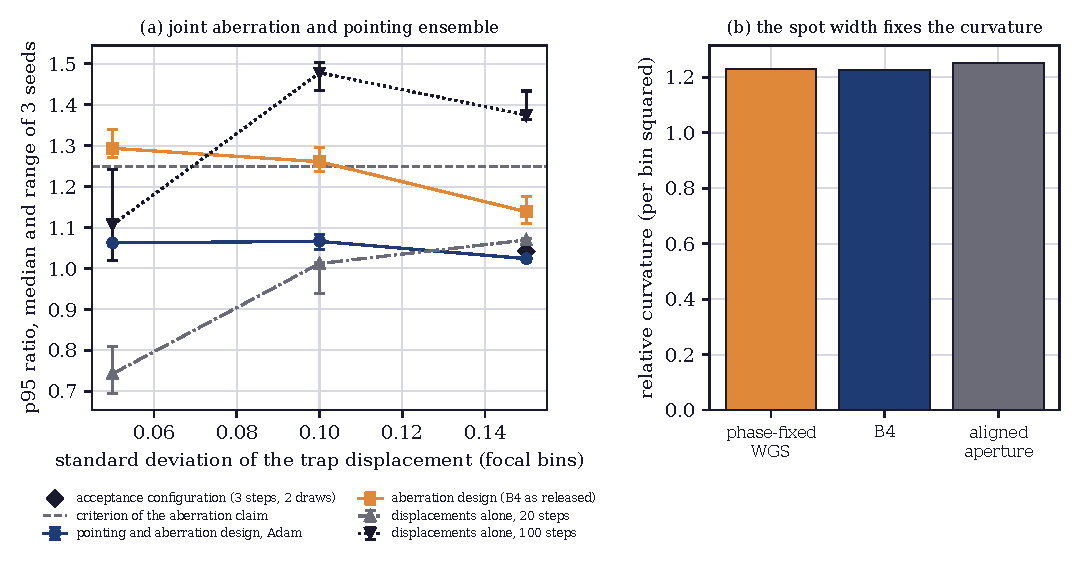
\includegraphics[width=\textwidth]{fig-pointing.pdf}
\caption{(a) Ratio of the 95th percentiles against the displacement for the joint ensemble (sample design and aberration design) and for displacements alone (20 and 100 steps); median and range of three seeds, with the acceptance configuration as a diamond. (b) Relative curvature of the trap intensity under displacement for phase-fixed WGS, the robust hologram and the aligned-aperture value of Proposition 4.}
\label{fig:pointing}
\end{figure}
